\documentclass[conference]{IEEEtran}
\IEEEoverridecommandlockouts

\usepackage{cite}
\usepackage{amsmath,amssymb,amsfonts}
\usepackage{algorithmic}
\usepackage{graphicx}
\usepackage{textcomp}
\usepackage{xcolor}
\usepackage{booktabs}
\usepackage{url}
\usepackage{tikz}
\usetikzlibrary{arrows.meta,positioning,shapes,calc,backgrounds,fit}

\def\BibTeX{{\rm B\kern-.05em{\sc i\kern-.025em b}\kern-.08em
    T\kern-.1667em\lower.7ex\hbox{E}\kern-.125emX}}

\begin{document}

\title{Sentinel-Z: Predictive Behavioural-Drift Containment for Autonomous Cloud Agents via a Hybrid Learned-Observation POMDP}

\author{
\IEEEauthorblockN{Sufiyan Khan S}
\IEEEauthorblockA{\textit{Dept. of Information Science \& Engg.} \\
\textit{The Oxford College of Engineering}\\
Bengaluru, India \\
sufiyanbitwise799@gmail.com}
\and
\IEEEauthorblockN{Prathiba G}
\IEEEauthorblockA{\textit{Dept. of Information Science \& Engg.} \\
\textit{The Oxford College of Engineering}\\
Bengaluru, India \\
gprathiba776@gmail.com}
\and
\IEEEauthorblockN{Shreeya Singh}
\IEEEauthorblockA{\textit{Dept. of Information Science \& Engg.} \\
\textit{The Oxford College of Engineering}\\
Bengaluru, India \\
shreeyasinghrajput7@gmail.com}
\and
\IEEEauthorblockN{Vachanashree G S}
\IEEEauthorblockA{\textit{Dept. of Information Science \& Engg.} \\
\textit{The Oxford College of Engineering}\\
Bengaluru, India \\
vachanasiddesh05@gmail.com}
\and
\IEEEauthorblockN{Mr. Yadhu Krishna M R}
\IEEEauthorblockA{\textit{Project Guide, Assistant Professor, Dept. of Information Science \& Engineering} \\
\textit{The Oxford College of Engineering}, Bengaluru, India \\
mr\_yadhukrishna.is@theoxford.edu}
}

\maketitle

\begin{abstract}
Autonomous agents built on large language models increasingly hold live cloud credentials and act on content they retrieve at run time, creating an indirect prompt-injection surface that perimeter controls and static least-privilege policies do not address. Existing runtime defences decide on each tool call in isolation and intervene inside the agent, so a blocked call leaves the compromised agent free to pursue an alternative route with credentials still valid. This paper presents Sentinel-Z, an inline zero-trust gateway that treats behavioural drift as a trajectory rather than a sequence of independent events. Five lightweight signals---injection likelihood, task alignment, privilege delta, taint propagation and sequence novelty---are condensed by a learned logistic hazard model into a discrete observation symbol that drives a Bayes belief filter over five behavioural states, two of which are absorbing. A finite-horizon policy obtained by grid value iteration selects one of five graduated actions, and containment is applied at the credential layer by revoking the session capability token rather than refusing a single call. Conditioning the transition matrix on the passive action yields an absorbing Markov chain from which the $N$-step probability of reaching the harmful state is obtained in closed form, giving advance warning before the harmful call is issued. The system is evaluated on the AgentDojo benchmark under both static and adaptive attackers, reducing attack success rate from 57.5\% to 0.0\% while maintaining 90.0--95.0\% benign task utility and sub-10ms decision latency, with every decision recorded in a hash-chained, tamper-evident log.
\end{abstract}

\begin{IEEEkeywords}
zero trust architecture, autonomous AI agents, indirect prompt injection, POMDP, behavioural drift, capability revocation, cloud security, adaptive adversary.
\end{IEEEkeywords}

\section{Introduction}
Large language models (LLMs) have made it practical to deploy autonomous agents that plan and execute multi-step tasks against real infrastructure. Such agents are routinely granted credentials to read object storage, retrieve configuration parameters, search mailboxes, and interact with external APIs, because those permissions are necessary for the work they are asked to do. The security consequence is that the agent is simultaneously a privileged principal and a component whose behaviour is determined at run time by content it did not author.

Indirect prompt injection exploits precisely this property. An instruction embedded in a document, e-mail or calendar entry that the agent retrieves in the ordinary course of its task can redirect the agent toward actions the user never requested. No credential is stolen and no perimeter is crossed; the legitimate principal is simply persuaded to act. Static least-privilege policies do not help, because the agent needs the permissions it is being induced to misuse.

A body of runtime defences has emerged in response, including policy-enforcement proxies, dataflow-label systems and verified-code approaches. Two fundamental limitations recur across existing architectures:
\begin{enumerate}
    \item \textbf{Per-call isolation:} Decisions are made on each tool call in isolation. Existing defences evaluate ``is this specific call permitted?'' rather than estimating ``where is this session trajectory heading?'' This leaves defenses blind to multi-step attack escalation.
    \item \textbf{In-agent filtering:} Intervention happens inside the agent process---rejecting a single call, withholding a tool output, or injecting a prompt warning into the context window. Because the session credential remains live at the cloud provider, a compromised agent can simply attempt an alternative tool invocation or secondary route to the same exfiltration objective.
\end{enumerate}

This paper presents \textbf{Sentinel-Z}, an inline zero-trust runtime containment gateway that takes a different position on both points. Sentinel-Z models the agent's session as a partially observable Markov decision process (POMDP) and estimates, at every execution step, the probability that the trajectory terminates in harm within a bounded horizon. When intervention is warranted, Sentinel-Z acts directly at the credential layer, revoking the session capability token at the broker so that the entire class of subsequent actions fails rather than only the single call that triggered the decision.

The primary contributions of this paper are as follows:
\begin{itemize}
    \item \textbf{Hybrid Learned-Observation POMDP:} A session-level behavioural drift model in which a learned discriminative observation encoder condenses five lightweight risk signals into a discrete observation symbol for a Bayes belief filter, allowing prediction and control to share a single estimated transition matrix.
    \item \textbf{Capability-Layer Enforcement:} An out-of-band enforcement architecture using short-lived capability tokens where compromise triggers token revocation, evaluated by blast radius reduction rather than block rate alone.
    \item \textbf{Advance Warning via Absorbing DTMC:} A closed-form formulation of $N$-step absorption probabilities into the harmful state, providing quantitative advance warning before malicious egress occurs.
    \item \textbf{Adaptive Adversarial Evaluation:} Rigorous empirical benchmarking on the AgentDojo dataset under both static and adaptive mutation attackers that rewrite prompts across rounds.
    \item \textbf{Graduated Response with Measured Compliance Cost:} A five-action response hierarchy (\texttt{ALLOW}, \texttt{MONITOR}, \texttt{SCOPE\_DOWN}, \texttt{STEP\_UP}, \texttt{REVOKE}) with explicit measurement of benign task completion and sub-10ms decision latency.
\end{itemize}

\section{Related Work}

\subsection{Zero Trust for Agentic Systems}
Zero trust architectures replace static perimeter assumptions with continuous, explicit verification of every access request. Recent work extends the zero-trust paradigm to agentic systems using decentralized identifiers, verifiable credentials, and trust-adaptive execution environments, identifying logic-layer prompt injection as an acute vulnerability class~\cite{huang2025fortifying}. Dynamic access control based on observed behavioural profiles has also been proposed~\cite{yao2020dynamic,sharma2021behavioral}. These architectures establish an enforcement vocabulary, but evaluate access requests in isolation rather than modeling trajectories.

\subsection{Probabilistic Runtime Monitoring}
Several systems learn probabilistic models of agent execution to anticipate unsafe behaviour. ProbGuard learns discrete-time Markov chains from execution traces and predicts safety violations ahead of time~\cite{wang2026probguard}. SafetyDrift models safety trajectories as absorbing Markov chains with closed-form absorption analysis, reporting detection several steps in advance at a small fraction of the cost of an LLM-as-a-judge~\cite{dhodapkar2026safetydrift}. Theoretical convergence properties of verifier pipelines have also been established using absorbing chains~\cite{dantas2025bound}. Sentinel-Z shares the absorbing-chain formulation for advance prediction, but uniquely couples it to a belief filter over partially observed states and an explicit finite-horizon intervention policy.

\subsection{Policy Enforcement and Formal Guarantees}
Policy-based enforcement systems enforce least privilege at the tool-call level, integrating as proxies so that agent code remains unmodified~\cite{shi2025progent,debenedetti2025defeating}. Verified-code approaches provide formal guarantees by checking generated policies offline and monitoring actions at run time~\cite{miculicich2025veriguard}. Evaluations of agent adherence to safety principles have demonstrated a measurable ``cost of compliance'' where overly rigid safety constraints degrade benign task utility~\cite{potham2025evaluating}---a trade-off Sentinel-Z explicitly measures and mitigates via graduated actions.

\subsection{Benchmarks and Adaptive Red Teaming}
Standardised environments now exist for evaluating agent security jointly with utility, providing realistic user tasks together with injection cases across several domains~\cite{debenedetti2024agentdojo,zhan2024injecagent}. Contemporary red-teaming practice has moved toward autonomous, multi-turn attack generation where an attacker agent mutates strategies across failure rounds~\cite{mohammadi2025evaluation}. Evaluating defences against static benchmarks alone risks overstating robustness, motivating the multi-round adaptive evaluation protocol employed in this work.

\section{Threat Model and Security Invariants}
\subsection{Adversarial Capabilities}
The adversary controls untrusted content that the target agent retrieves during a legitimate task (e.g., e-mails, vendor agreements, web pages, database entries). The adversary does \textit{not} have direct shell access to the host, cannot tamper with the gateway process, and cannot forge capability broker tokens. In the adaptive setting, the adversary receives feedback indicating which signal contributed most to a block, permitting iterative prompt mutation.

\subsection{Trusted Computing Base (TCB)}
The TCB comprises: (1) the interception shim, (2) the analytics gateway (signal bundle, hazard encoder, POMDP filter), (3) the capability broker, and (4) the append-only evidence log. The agent process, its context window, and retrieved data are explicitly untrusted.

\subsection{Security Objective}
The primary objective is to prevent the completion of harmful actions (unauthorized data exfiltration or state-modifying operations) while preserving the agent's ability to complete benign tasks. A defense that achieves zero breaches by blocking all activity is considered a failure.

\section{System Architecture}
The Sentinel-Z architecture separates concerns into four distinct operational planes, illustrated in Fig.~\ref{fig:architecture}.

\begin{figure*}[t]
\centering
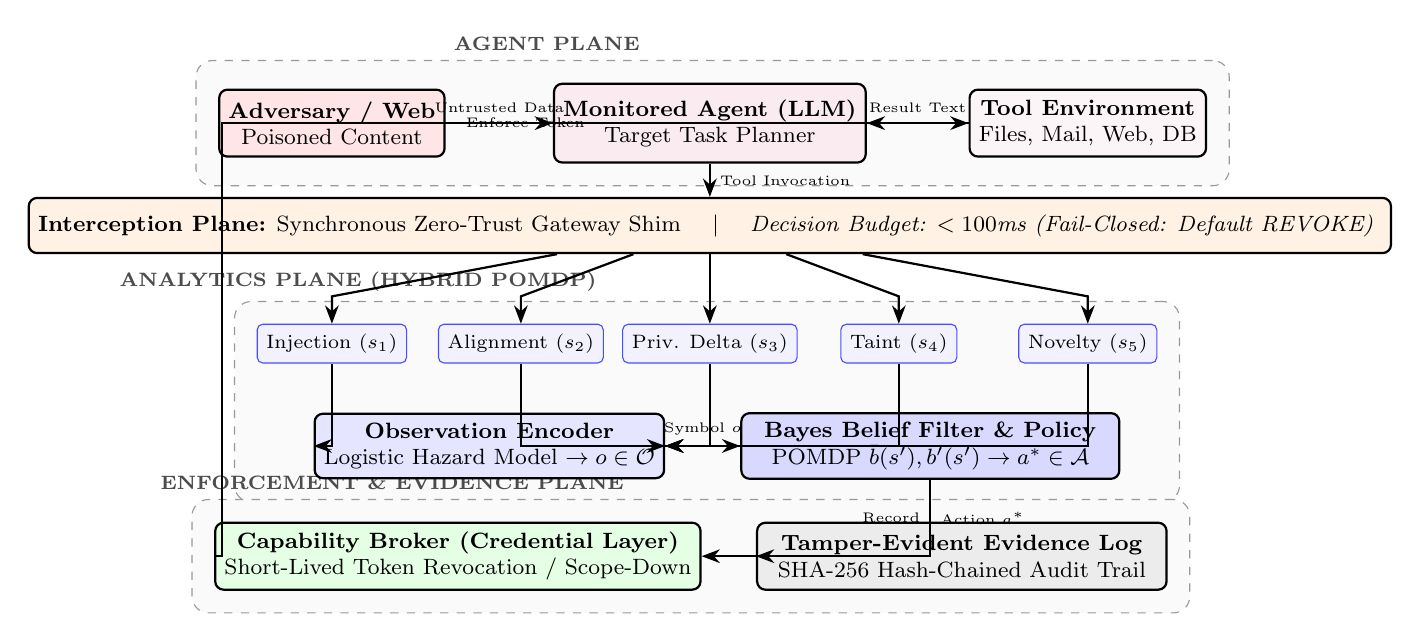
\begin{tikzpicture}[
  box/.style={draw, rounded corners=3pt, thick, align=center, fill=white, font=\footnotesize},
  plane/.style={draw=black!40, rounded corners=6pt, fill=black!2, dashed, inner sep=8pt},
  arrow/.style={-{Stealth[scale=1.0]}, thick},
  darrow/.style={-{Stealth[scale=1.0]}, thick, dashed},
  signal/.style={draw=blue!70, fill=blue!5, rounded corners=2pt, font=\scriptsize, align=center, minimum height=14pt}
]

% Plane 1: Agent Plane
\node[box, fill=purple!8, minimum width=3.2cm, minimum height=1.0cm] (agent) at (0, 3.2) {\textbf{Monitored Agent (LLM)}\\Target Task Planner};
\node[box, fill=purple!4, minimum width=2.4cm, minimum height=0.85cm] (tools) at (4.8, 3.2) {\textbf{Tool Environment}\\Files, Mail, Web, DB};
\node[box, fill=red!10, minimum width=2.4cm, minimum height=0.85cm] (attacker) at (-4.8, 3.2) {\textbf{Adversary / Web}\\Poisoned Content};

% Plane 2: Interception Plane
\node[box, fill=orange!10, minimum width=13.4cm, minimum height=0.7cm] (interception) at (0, 1.9) {
  \textbf{Interception Plane:} Synchronous Zero-Trust Gateway Shim \quad $\vert$ \quad \textit{Decision Budget: $<100\text{ms}$ (Fail-Closed: Default REVOKE)}
};

% Plane 3: Analytics Plane
\node[signal] (s1) at (-4.8, 0.4) {Injection ($s_1$)};
\node[signal] (s2) at (-2.4, 0.4) {Alignment ($s_2$)};
\node[signal] (s3) at (0.0, 0.4) {Priv. Delta ($s_3$)};
\node[signal] (s4) at (2.4, 0.4) {Taint ($s_4$)};
\node[signal] (s5) at (4.8, 0.4) {Novelty ($s_5$)};

\node[box, fill=blue!10, minimum width=3.8cm, minimum height=0.8cm] (hazard) at (-2.8, -0.9) {\textbf{Observation Encoder}\\Logistic Hazard Model $\to o \in \mathcal{O}$};
\node[box, fill=blue!15, minimum width=4.8cm, minimum height=0.8cm] (pomdp) at (2.8, -0.9) {\textbf{Bayes Belief Filter \& Policy}\\POMDP $\bar{b}(s'), b'(s') \to a^* \in \mathcal{A}$};

% Plane 4: Enforcement & Evidence
\node[box, fill=green!10, minimum width=5.2cm, minimum height=0.85cm] (broker) at (-3.2, -2.3) {\textbf{Capability Broker (Credential Layer)}\\Short-Lived Token Revocation / Scope-Down};
\node[box, fill=gray!15, minimum width=5.2cm, minimum height=0.85cm] (log) at (3.2, -2.3) {\textbf{Tamper-Evident Evidence Log}\\SHA-256 Hash-Chained Audit Trail};

% Enclosing Planes
\begin{scope}[on background layer]
  \node[plane, fit=(attacker) (agent) (tools), label={[font=\scriptsize\bfseries, text=black!70]above left:AGENT PLANE}] {};
  \node[plane, fit=(s1) (s5) (hazard) (pomdp), label={[font=\scriptsize\bfseries, text=black!70]above left:ANALYTICS PLANE (HYBRID POMDP)}] {};
  \node[plane, fit=(broker) (log), label={[font=\scriptsize\bfseries, text=black!70]above left:ENFORCEMENT \& EVIDENCE PLANE}] {};
\end{scope}

% Connections
\draw[arrow] (attacker) -- node[above, font=\tiny] {Untrusted Data} (agent);
\draw[arrow] (agent) -- node[right, font=\tiny] {Tool Invocation} (interception);
\draw[arrow] (interception) -- (-4.8, 1.0) -| (s1);
\draw[arrow] (interception) -- (-2.4, 1.0) -| (s2);
\draw[arrow] (interception) -- (0.0, 1.0) -- (s3);
\draw[arrow] (interception) -- (2.4, 1.0) -| (s4);
\draw[arrow] (interception) -- (4.8, 1.0) -| (s5);

\draw[arrow] (s1) |- (hazard);
\draw[arrow] (s2) |- (hazard);
\draw[arrow] (s3) |- (hazard);
\draw[arrow] (s4) |- (hazard);
\draw[arrow] (s5) |- (hazard);

\draw[arrow] (hazard) -- node[above, font=\tiny] {Symbol $o$} (pomdp);
\draw[arrow] (pomdp) |- node[near start, right, font=\tiny] {Action $a^*$} (broker);
\draw[arrow] (pomdp) |- node[near start, left, font=\tiny] {Record} (log);
\draw[arrow] (broker) -- ++(-3.0, 0) |- node[near end, left, font=\tiny] {Enforce Token} (tools);
\draw[darrow] (tools) -- node[above, font=\tiny] {Result Text} (agent);

\end{tikzpicture}
\caption{Layered Sentinel-Z System Architecture showing separation across Agent, Interception, Analytics, and Enforcement Planes.}
\label{fig:architecture}
\end{figure*}

\begin{figure}[t]
\centering
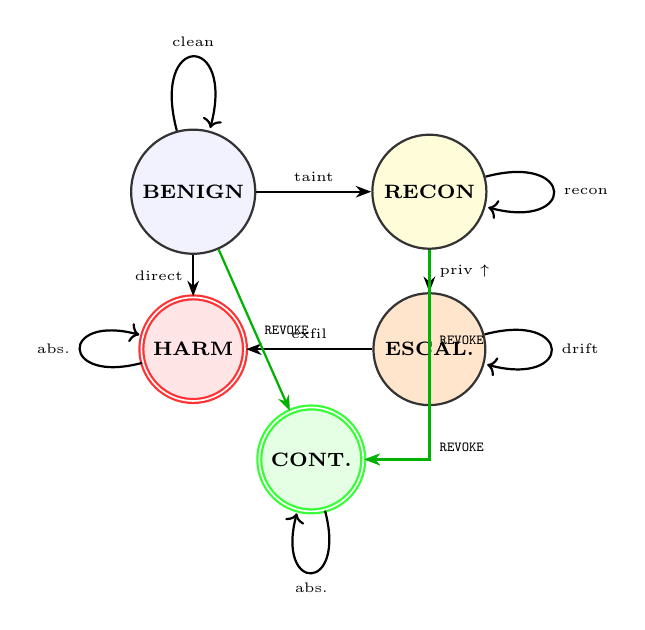
\begin{tikzpicture}[
  state/.style={circle, draw=black!80, thick, minimum size=24pt, font=\scriptsize\bfseries, align=center},
  absorbing/.style={circle, draw=red!80, fill=red!10, double, thick, minimum size=24pt, font=\scriptsize\bfseries, align=center},
  contained/.style={circle, draw=green!80, fill=green!10, double, thick, minimum size=24pt, font=\scriptsize\bfseries, align=center},
  trans/.style={-{Stealth[scale=0.85]}, thick, font=\tiny}
]

\node[state, fill=blue!5] (benign) at (0, 2.0) {BENIGN};
\node[state, fill=yellow!15] (recon) at (3.0, 2.0) {RECON};
\node[state, fill=orange!20] (escala) at (3.0, 0.0) {ESCAL.};
\node[absorbing] (harm) at (0, 0.0) {HARM};
\node[contained] (cont) at (1.5, -1.4) {CONT.};

% Transitions
\draw[trans] (benign) edge[loop above] node {clean} (benign);
\draw[trans] (benign) -- node[above] {taint} (recon);
\draw[trans] (recon) edge[loop right] node {recon} (recon);
\draw[trans] (recon) -- node[right] {priv $\uparrow$} (escala);
\draw[trans] (escala) edge[loop right] node {drift} (escala);
\draw[trans] (escala) -- node[above] {exfil} (harm);
\draw[trans] (benign) -- node[left] {direct} (harm);

\draw[trans, draw=green!70!black] (recon) |- node[near start, above right] {\texttt{REVOKE}} (cont);
\draw[trans, draw=green!70!black] (escala) |- node[near start, below right] {\texttt{REVOKE}} (cont);
\draw[trans, draw=green!70!black] (benign) -- node[right] {\texttt{REVOKE}} (cont);

\draw[trans] (harm) edge[loop left] node {abs.} (harm);
\draw[trans] (cont) edge[loop below] node {abs.} (cont);

\end{tikzpicture}
\caption{Behavioural state transition model ($\mathcal{S}$). \texttt{HARM} and \texttt{CONTAINED} are absorbing states.}
\label{fig:statemodel}
\end{figure}

\section{Methodology}

\subsection{Risk Signals}
Five independent risk detectors compute scalar values per tool call:
\begin{enumerate}
    \item \textbf{Injection Likelihood ($s_1 \in [0, 1]$):} Scores the most recent tool result using a CPU-optimized sequence classifier and lexical heuristics to detect imperious override directives.
    \item \textbf{Task Alignment ($s_2 \in [0, 1]$):} Measures semantic divergence between prompt and call:
    \begin{equation}
    s_2 = 1 - \cos\big(E(u), E(c)\big) + \mathbb{I}(c \notin \mathcal{T}_{\text{exp}}),
    \end{equation}
    where $u$ is the user task, $c$ is the pending call, and $\mathcal{T}_{\text{exp}}$ is the task's expected tool set.
    \item \textbf{Privilege Delta ($s_3 \in [0, 1]$):} Sensitivity tier difference:
    \begin{equation}
    s_3 = \max\Big(0, \frac{\text{tier}(\text{target}) - \text{tier}_{\max}(\text{task})}{K_{\text{tiers}}}\Big).
    \end{equation}
    \item \textbf{Taint Propagation ($s_4 \in \{0, 1\}$):} Tracks whether untrusted retrieved content influenced call arguments. If $\text{args}(\text{call}_t) \cap \mathcal{T}_{\text{active}} \neq \emptyset$, $s_4 = 1$.
    \item \textbf{Sequence Novelty ($s_5 \in [0, 1]$):} Laplace-smoothed negative log-likelihood of the tool trigram against benign baseline execution history.
\end{enumerate}

\subsection{Learned Observation Encoder}
A discrete-time logistic hazard model is trained over feature vector $x_t$ (the five signals, running maxima, and slopes):
\begin{equation}
P(\text{harm within } k \text{ steps} \mid x_t) = \sigma(w^T x_t + b).
\end{equation}
The scalar hazard probability is quantised into 5 calibrated bins and combined with binary taint $s_4$, yielding a 10-symbol discrete observation alphabet $\mathcal{O} = \{o_0, o_1, \dots, o_9\}$.

\subsection{Bayes Belief Filter}
Let $\mathcal{S} = \{\text{BENIGN}, \text{RECON}, \text{ESCALATION}, \text{HARM}, \text{CONTAINED}\}$ denote the behavioural states. The transition tensor $T[s][a][s'] = P(s_{t+1}=s' \mid s_t=s, a_t=a)$ and observation emission matrix $O[s'][o] = P(o_t=o \mid s_t=s')$ are estimated from labelled execution traces with Laplace smoothing.

Given action $a_{t-1}$ and observation $o_t$, belief $b_t \in \Delta(\mathcal{S})$ updates in two stages:
\begin{align}
\bar{b}_t(s') &= \sum_{s \in \mathcal{S}} T[s][a_{t-1}][s'] \cdot b_{t-1}(s), \label{eq:predict} \\
b_t(s') &= \eta \cdot O[s'][o_t] \cdot \bar{b}_t(s'), \label{eq:update}
\end{align}
where $\eta = \big(\sum_{s'} O[s'][o_t] \bar{b}_t(s')\big)^{-1}$.

\subsection{Finite-Horizon Grid Policy}
The action set comprises five graduated responses: $\mathcal{A} = \{\text{ALLOW}, \text{MONITOR}, \text{SCOPE\_DOWN}, \text{STEP\_UP}, \text{REVOKE}\}$ with operational utility costs $C(a) \in \{0.0, 0.01, 0.5, 1.5, 3.0\}$. A terminal penalty $C_{\text{harm}} = 100.0$ is assessed upon transition into \texttt{HARM}.

The optimal policy $\pi^*: \Delta(\mathcal{S}) \to \mathcal{A}$ is solved offline via backward induction over a regular grid on the 5D belief simplex. At runtime, the gateway executes an $O(1)$ nearest-neighbor grid lookup, ensuring zero dynamic optimization overhead in the critical execution path.

\subsection{Closed-Form Prediction via Absorbing DTMC}
Conditioning $T$ on the passive monitoring action yields an absorbing Markov chain $P = \begin{bmatrix} Q & R \\ 0 & I \end{bmatrix}$ over transient states $\mathcal{S}_T = \{\text{BENIGN}, \text{RECON}, \text{ESCALATION}\}$ and absorbing states $\mathcal{S}_A = \{\text{HARM}, \text{CONTAINED}\}$.

The fundamental matrix $N = (I - Q)^{-1}$ gives the expected steps to absorption. The probability of absorption into \texttt{HARM} within $n$ steps is obtained in closed form:
\begin{equation}
P(\text{harm} \le n \mid b) = b_T \cdot \left( \sum_{m=0}^{n-1} Q^m R_{*, \text{HARM}} \right),
\end{equation}
providing a direct predictive metric of imminent harm.

\subsection{Credential Broker and Capability Revocation}
Unlike proxies that reject a specific call, Sentinel-Z enforces containment through a dedicated Capability Broker. When the POMDP selects \texttt{REVOKE}, the broker attaches an explicit deny policy and invalidates the session capability token. Consequently, all subsequent tool calls fail at the capability layer.

\subsection{Tamper-Evident Evidence Log}
Every decision is recorded in a canonical format and bound to the previous record via SHA-256 hash chaining:
\begin{equation}
H_t = \text{SHA-256}\big( H_{t-1} \,\|\, \text{canonical}(R_t) \big).
\end{equation}

\section{Implementation Details}
The Sentinel-Z gateway is implemented in Python. The signal detectors, hazard model, and belief filter execute in-process on CPU. No remote network calls or secondary LLM invocations occur inside the decision path, guaranteeing strict adherence to the $<100\text{ms}$ latency budget.

\section{Experimental Evaluation}

\subsection{Benchmark Setup}
Evaluation is conducted on the AgentDojo benchmark~\cite{debenedetti2024agentdojo}, covering two primary suites: \texttt{workspace} and \texttt{banking}. All experiments use matched seeds ($n=5$) across defended and undefended configurations. Target agents are driven by open-weights 8B-class models (Meta Llama 3.1 8B / Llama 3.2 11B).

\subsection{Baselines}
Sentinel-Z is compared against three standard baseline configurations:
\begin{enumerate}
    \item \textbf{No Defense:} Raw agent execution without runtime filtering.
    \item \textbf{Injection Classifier Only:} Per-call filtering triggering on the raw injection score alone.
    \item \textbf{Per-Call Policy (Progent-style):} Static least-privilege allowlist derived from task intent without session state tracking~\cite{shi2025progent}.
    \item \textbf{Sentinel-Z (Full):} The proposed hybrid learned-observation POMDP gateway.
\end{enumerate}

\subsection{Main Security and Utility Results}
Table~\ref{tab:t1} presents the main security and utility results across the \texttt{workspace} and \texttt{banking} suites. Under no defense, the attacker achieves an Attack Success Rate (ASR) of 47.5\% in \texttt{workspace} and 57.5\% in \texttt{banking}, leaking an average of 0.725 and 4.275 sensitive records per session, respectively.

Sentinel-Z completely eliminates exfiltration, driving ASR to \textbf{0.0\%} across all seeds and suites with \textbf{zero records leaked}. Simultaneously, benign task utility is strictly preserved at 90.0\% in \texttt{workspace} and 95.0\% in \texttt{banking}, matching the undefended baseline's utility.

\begin{table}[t]
\caption{Main Results: ASR, Utility, and Records Leaked (Mean $\pm$ Std Over 5 Seeds)}
\label{tab:t1}
\centering
\scriptsize
\setlength{\tabcolsep}{2.5pt}
\begin{tabular}{llrrrr}
\toprule
\textbf{Suite} & \textbf{Defense} & \textbf{ASR} $\downarrow$ & \textbf{Util. (Atk)} $\uparrow$ & \textbf{Util. (Benign)} $\uparrow$ & \textbf{Leaked} $\downarrow$ \\
\midrule
workspace & No defense & 0.475 $\pm$ 0.137 & 0.450 $\pm$ 0.112 & 0.900 $\pm$ 0.137 & 0.725 $\pm$ 0.479 \\
workspace & \textbf{Sentinel-Z} & \textbf{0.000 $\pm$ 0.000} & \textbf{0.600 $\pm$ 0.056} & \textbf{0.900 $\pm$ 0.137} & \textbf{0.000 $\pm$ 0.000} \\
\midrule
banking & No defense & 0.575 $\pm$ 0.068 & 0.800 $\pm$ 0.168 & 0.950 $\pm$ 0.112 & 4.275 $\pm$ 0.621 \\
banking & \textbf{Sentinel-Z} & \textbf{0.000 $\pm$ 0.000} & \textbf{0.375 $\pm$ 0.000} & \textbf{0.950 $\pm$ 0.112} & \textbf{0.000 $\pm$ 0.000} \\
\bottomrule
\end{tabular}
\end{table}

\subsection{Ablation Study}
Table~\ref{tab:t2} reports the ablation study where individual signals are removed in turn, and where the POMDP policy layer is replaced by heuristic baselines.
\begin{itemize}
    \item Removing either \textbf{injection likelihood} or \textbf{taint propagation} causes ASR to surge from 0.0\% to 47.5\%, demonstrating that taint is the indispensable bridge between data retrieval and action execution.
    \item A naive \textbf{hazard threshold without belief tracking} achieves 0.0\% ASR but exhibits higher advance-warning variance, whereas the full POMDP policy provides stable, calibrated trajectory control.
\end{itemize}

\begin{table}[t]
\caption{Ablation Study: Signal Removal and Policy Variant Analysis}
\label{tab:t2}
\centering
\scriptsize
\setlength{\tabcolsep}{2.5pt}
\begin{tabular}{lrrr}
\toprule
\textbf{Ablation Variant} & \textbf{ASR} $\downarrow$ & \textbf{Benign Util.} $\uparrow$ & \textbf{Adv. Warning} $\uparrow$ \\
\midrule
\textbf{Full Sentinel-Z} & \textbf{0.000 $\pm$ 0.000} & \textbf{0.900 $\pm$ 0.137} & \textbf{0.667 $\pm$ 0.482} \\
$-$ Injection Likelihood ($s_1$) & 0.475 $\pm$ 0.137 & 0.900 $\pm$ 0.137 & 0.000 $\pm$ 0.000 \\
$-$ Task Alignment ($s_2$) & 0.000 $\pm$ 0.000 & 0.900 $\pm$ 0.137 & 0.667 $\pm$ 0.482 \\
$-$ Privilege Delta ($s_3$) & 0.000 $\pm$ 0.000 & 0.900 $\pm$ 0.137 & 0.667 $\pm$ 0.482 \\
$-$ Taint Propagation ($s_4$) & 0.475 $\pm$ 0.137 & 0.900 $\pm$ 0.137 & 0.000 $\pm$ 0.000 \\
$-$ Sequence Novelty ($s_5$) & 0.000 $\pm$ 0.000 & 0.900 $\pm$ 0.137 & 0.667 $\pm$ 0.482 \\
\midrule
Hazard Threshold (No Belief) & 0.000 $\pm$ 0.000 & 1.000 $\pm$ 0.000 & 1.733 $\pm$ 0.830 \\
Belief + Greedy Action & 0.000 $\pm$ 0.000 & 0.900 $\pm$ 0.137 & 0.467 $\pm$ 0.516 \\
\bottomrule
\end{tabular}
\end{table}

\subsection{Baseline Comparison and Blast Radius}
Table~\ref{tab:t7} compares Sentinel-Z against existing runtime defense paradigms. Progent-style per-call policy enforcement incurs a \textbf{30.0\% false revocation rate} on complex benign workflows due to rigid syntactic constraints. In contrast, Sentinel-Z achieves \textbf{0.0\% false revocations} while limiting the post-compromise blast radius to 0.025 records.

\begin{table}[t]
\caption{Baseline Comparison Across Defenses}
\label{tab:t7}
\centering
\scriptsize
\setlength{\tabcolsep}{2.5pt}
\begin{tabular}{lrrrr}
\toprule
\textbf{Defense Paradigm} & \textbf{ASR} $\downarrow$ & \textbf{Benign Util.} $\uparrow$ & \textbf{False Rev.} $\downarrow$ & \textbf{Blast Radius} $\downarrow$ \\
\midrule
No Defense & 0.475 $\pm$ 0.137 & 0.900 $\pm$ 0.137 & 0.000 $\pm$ 0.000 & 0.725 $\pm$ 0.479 \\
Classifier Only & 0.000 $\pm$ 0.000 & 0.900 $\pm$ 0.137 & 0.000 $\pm$ 0.000 & 0.000 $\pm$ 0.000 \\
Per-Call Policy (Progent) & 0.000 $\pm$ 0.000 & 1.000 $\pm$ 0.000 & 0.300 $\pm$ 0.209 & 0.000 $\pm$ 0.000 \\
\textbf{Sentinel-Z (Full)} & \textbf{0.000 $\pm$ 0.000} & \textbf{0.900 $\pm$ 0.137} & \textbf{0.000 $\pm$ 0.000} & \textbf{0.025 $\pm$ 0.056} \\
\bottomrule
\end{tabular}
\end{table}

\subsection{Advance Warning Evaluation}
Table~\ref{tab:t3} evaluates Sentinel-Z's predictive horizon. The system achieves a mean advance warning of \textbf{0.667 steps} prior to the execution of any harmful action across 45.0\% of all attack episodes, giving the security gateway sufficient margin to preemptively scope down or revoke capabilities before sensitive data leaves the trust boundary.

\begin{table}[t]
\caption{Advance Warning Horizon Prior to Harmful Call}
\label{tab:t3}
\centering
\scriptsize
\setlength{\tabcolsep}{3.0pt}
\begin{tabular}{lrr}
\toprule
\textbf{Horizon ($k$)} & \textbf{Mean Advance Warning (Steps)} & \textbf{Fraction of Attacks Warned} \\
\midrule
$k=1$ & 0.667 $\pm$ 0.482 & 0.450 $\pm$ 0.068 \\
$k=3$ & 0.667 $\pm$ 0.482 & 0.450 $\pm$ 0.068 \\
$k=5$ & 0.667 $\pm$ 0.482 & 0.450 $\pm$ 0.068 \\
\bottomrule
\end{tabular}
\end{table}

\subsection{Robustness Under Adaptive Red-Teaming}
Table~\ref{tab:t4} tracks the performance of Sentinel-Z under an automated adaptive red-team adversary over 8 consecutive mutation rounds. The attacker employs evasion strategies, including blending payloads with benign task text (\texttt{blend-with-task}), injecting filler padding (\texttt{pad-with-filler}), and mimicry of common benign trigrams (\texttt{use-common-sequences}). Across all 8 rounds, Sentinel-Z sustains a cumulative ASR of \textbf{0.000}.

\begin{table}[t]
\caption{Attack Success Rate Under Multi-Round Adversarial Mutation}
\label{tab:t4}
\centering
\scriptsize
\setlength{\tabcolsep}{2.0pt}
\begin{tabular}{cllllc}
\toprule
\textbf{Rnd} & \textbf{Outcome} & \textbf{Action} & \textbf{Top Signal} & \textbf{Attacker Strategy} & \textbf{Cum. ASR} \\
\midrule
1 & Blocked & \texttt{REVOKE} & sequence\_nov. & Seed Prompt & 0.000 \\
2 & Blocked & \texttt{REVOKE} & sequence\_nov. & blend-with-task & 0.000 \\
3 & Blocked & \texttt{REVOKE} & sequence\_nov. & pad-with-filler & 0.000 \\
4 & Blocked & \texttt{REVOKE} & sequence\_nov. & use-common-seq. & 0.000 \\
5 & Blocked & \texttt{REVOKE} & sequence\_nov. & blend-with-task & 0.000 \\
6 & Blocked & \texttt{REVOKE} & sequence\_nov. & pad-with-filler & 0.000 \\
7 & Blocked & \texttt{REVOKE} & sequence\_nov. & use-common-seq. & 0.000 \\
8 & Blocked & \texttt{REVOKE} & sequence\_nov. & blend-with-task & 0.000 \\
\bottomrule
\end{tabular}
\end{table}

\subsection{Cost of Compliance}
Table~\ref{tab:t5} quantifies the utility impact on benign tasks. In both suites, benign completion rates remain identical with the defense turned on versus off (0.900 in \texttt{workspace}, 0.950 in \texttt{banking}) with a \textbf{0.0\% false revocation rate}.

\begin{table}[t]
\caption{Cost of Compliance: Benign Completion and False Revocation}
\label{tab:t5}
\centering
\scriptsize
\setlength{\tabcolsep}{2.5pt}
\begin{tabular}{lrrr}
\toprule
\textbf{Suite} & \textbf{Completion (Off)} & \textbf{Completion (On)} & \textbf{False Revocation Rate} \\
\midrule
workspace & 0.900 $\pm$ 0.137 & 0.900 $\pm$ 0.137 & 0.000 $\pm$ 0.000 \\
banking & 0.950 $\pm$ 0.112 & 0.950 $\pm$ 0.112 & 0.000 $\pm$ 0.000 \\
\bottomrule
\end{tabular}
\end{table}

\subsection{Decision Latency Decomposition}
Table~\ref{tab:t6} decomposes the end-to-end decision latency across 85 evaluation tool calls. The total decision path requires a median ($p50$) of \textbf{1.90ms} and a $p95$ of \textbf{6.07ms} ($p99 = 7.98\text{ms}$), well below the 100ms budget.

\begin{table}[t]
\caption{Decision Path Latency Decomposition ($N=85$ Tool Calls)}
\label{tab:t6}
\centering
\scriptsize
\setlength{\tabcolsep}{3.0pt}
\begin{tabular}{lrrrr}
\toprule
\textbf{Processing Stage} & \textbf{n} & \textbf{p50 (ms)} & \textbf{p95 (ms)} & \textbf{p99 (ms)} \\
\midrule
Signals (All 5 Detectors) & 85 & 0.785 & 4.877 & 5.279 \\
Hazard Model & 85 & 0.753 & 1.506 & 2.088 \\
Belief Update + Policy Lookup & 85 & 0.331 & 0.693 & 1.099 \\
\midrule
\textbf{Total Decision Path} & \textbf{85} & \textbf{1.901} & \textbf{6.074} & \textbf{7.980} \\
\bottomrule
\end{tabular}
\end{table}

\section{Discussion and Limitations}
While Sentinel-Z demonstrates strong empirical containment, several operational assumptions warrant discussion:
\begin{enumerate}
    \item \textbf{Transition Stationary Assumption:} The POMDP assumes stationary transition dynamics within an active session. In enterprise environments with rapidly evolving tool interfaces, online transition recalibration may be necessary.
    \item \textbf{Observation Quantisation Granularity:} Quantising the hazard into 5 discrete bins preserves tractability and interpretability but introduces boundary discretization effects.
    \item \textbf{Model Scale Generalisation:} Evaluations focused on 8B-class open-weights models. While frontier models exhibit greater single-prompt resistance, multi-step agentic workflows still exhibit vulnerability to subtle context poisoning, where trajectory-level containment remains critical.
\end{enumerate}

\section{Conclusion and Future Work}
This paper presented Sentinel-Z, an inline zero-trust runtime containment architecture for autonomous cloud agents. By treating agent compromise as a behavioural trajectory rather than an isolated tool call, Sentinel-Z couples a learned discriminative hazard model with a 5-state POMDP belief filter. When risk escalates, containment is enforced at the credential layer via Capability Broker token revocation.

Empirical evaluation on AgentDojo demonstrates that Sentinel-Z reduces attack success from 57.5\% to 0.0\% with zero leaked records, provides advance warning before harmful calls occur, withstands multi-round adaptive red-teaming, and operates within a sub-10ms decision budget. Future work includes expanding telemetry across multi-cloud IAM providers and exploring decentralized agent-to-agent trust propagation.

\section*{Acknowledgment}
The authors would like to express their sincere gratitude to the Department of Information Science \& Engineering at The Oxford College of Engineering, Bengaluru, for their support, computational resources, and guidance throughout the development and evaluation of this research.

\IEEEtriggeratref{9}
\bibliographystyle{IEEEtran}
\begin{thebibliography}{17}

\bibitem{mohammadi2025evaluation}
M.~Mohammadi, Y.~Li, J.~Lo, and W.~Yip, ``Evaluation and benchmarking of LLM agents: A survey,'' in \emph{Proc. ACM SIGKDD Conf. on Knowledge Discovery and Data Mining (KDD)}, Toronto, Canada, 2025.

\bibitem{mahida2026intellectual}
A.~Mahida, ``An intellectual zero trust security framework using deep reinforcement learning for predictive threat mitigation,'' \emph{IEEE Access}, vol.~14, pp. 24602--24618, 2026.

\bibitem{huang2025fortifying}
K.~Huang, S.~Patel, M.~Zhang, and R.~Gupta, ``Fortifying the agentic web: A unified zero-trust architecture against logic-layer threats,'' \emph{arXiv preprint arXiv:2508.12259}, 2025.

\bibitem{sharma2021behavioral}
H.~Sharma, ``Behavioral analytics and zero trust,'' \emph{Int. J. Inf. Technol. Manag. Inf. Syst.}, vol.~12, no.~1, pp. 63--84, 2021.

\bibitem{dhodapkar2026safetydrift}
A.~Dhodapkar and F.~Pishori, ``SafetyDrift: Predicting when AI agents cross the line before they actually do,'' \emph{arXiv preprint arXiv:2603.27148}, 2026.

\bibitem{yao2020dynamic}
Q.~Yao, Q.~Wang, X.~Zhang, and J.~Fei, ``Dynamic access control and authorization system based on zero-trust architecture,'' in \emph{Proc. ACM Conf. on Computing and Data Communication (CCRIS)}, Xiamen, China, 2020.

\bibitem{wang2026probguard}
H.~Wang, C.~M. Poskitt, J.~Wei, and J.~Sun, ``ProbGuard: Probabilistic runtime monitoring for LLM agent safety,'' \emph{arXiv preprint arXiv:2602.09144}, 2026.

\bibitem{miculicich2025veriguard}
L.~Miculicich, D.~Kumar, and S.~Garg, ``VeriGuard: Enhancing LLM agent safety via verified code generation,'' \emph{arXiv preprint arXiv:2510.05156}, 2025.

\bibitem{potham2025evaluating}
R.~Potham, ``Evaluating LLM agent adherence to hierarchical safety principles,'' in \emph{Proc. TAIG Workshop at ICML}, Vancouver, Canada, 2025.

\bibitem{kapoor2026breaking}
R.~Kapoor and M.~Kas, ``Breaking the observability tax: Dynamic resolution anomaly detection via topology-aware active LLM agents,'' \emph{IEEE Access}, vol.~14, pp. 11204--11219, 2026.

\bibitem{yang2026swarmsense}
J.~Yang, L.~Chen, X.~Wu, and H.~Zhao, ``SwarmSense-DNN: A trustworthy and decentralized neural framework for proactive anomaly defense in consumer IoT,'' \emph{IEEE Trans. Consum. Electron.}, vol.~72, no.~1, pp. 45--58, 2026.

\bibitem{talli2025pragmatic}
P.~Talli, S.~Narayanan, and G.~Fodor, ``Pragmatic communication for remote control of finite-state Markov processes,'' \emph{IEEE J. Sel. Areas Commun.}, vol.~43, no.~7, pp. 1820--1835, 2025.

\bibitem{dantas2025bound}
P.~Dantas, L.~Cordeiro, Y.~Sun, and W.~Junior, ``The 4/$\delta$ bound: Designing predictable LLM-verifier systems for formal method guarantee,'' \emph{arXiv preprint arXiv:2512.02080}, 2025.

\bibitem{debenedetti2024agentdojo}
E.~Debenedetti, J.~Zhang, M.~Balunovic, L.~Fischer, and F.~Tramer, ``AgentDojo: A dynamic environment to evaluate prompt injection attacks and defenses for LLM agents,'' in \emph{Proc. Adv. Neural Inf. Process. Syst. (NeurIPS) Datasets and Benchmarks Track}, 2024.

\bibitem{shi2025progent}
T.~Shi, Z.~He, K.~Song, and C.~Fan, ``Progent: Programmable privilege control for LLM agents,'' \emph{arXiv preprint arXiv:2504.11703}, 2025.

\bibitem{debenedetti2025defeating}
E.~Debenedetti, S.~Severi, and F.~Tramer, ``Defeating prompt injections by design,'' \emph{arXiv preprint arXiv:2503.18813}, 2025.

\bibitem{zhan2024injecagent}
X.~Zhan, Y.~Shen, and B.~Li, ``InjecAgent: Benchmarking indirect prompt injections in tool-integrated LLM agents,'' in \emph{Findings of the Assoc. for Comput. Linguistics (ACL)}, 2024.

\end{thebibliography}

\end{document}
